\chapter{The Alarm Screen}
\section{Overview}
The Alarm Screen is the screen the Operator uses to diagnose the Saw when it is in a Faulted State. It will provide information to the Operator about the nature of the Fault, and allow for acknowledgement of the faulted state by the Operator.
\begin{figure}
	\centering
	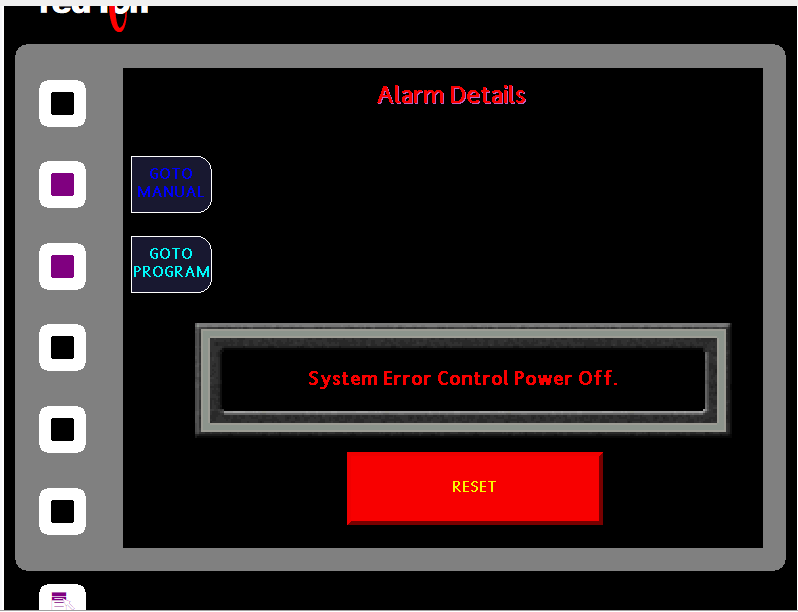
\includegraphics[width=0.5
	\linewidth]{screen-captures/alarms}
	\caption{Alarm Screen}
	\label{fig:alarm-screen}
\end{figure}
\pagebreak
\section{Alarm Screen Details}
The Alarm Screen details are divided into the following general categories.
\begin{list}{$\diamond$}{}
	\item \textbf{Screen Navigation}
	\item \textbf{Alarm Message Centre}
	\item \textbf{Alarm Acknowledge/Reset}
\end{list}
\subsection{Screen Navigation}Is performed by using the programmable Function Keys (FKeys) located down the left hand side of the OI Terminal (refer to Figure 2.2). The Operator may navigate to the \textbf{\textit{Manual Screen}} and the \textbf{\textit{Program Screen}}. and of course the \textbf{\textit{Main Screen}} using the \textit{Menu} FKey.
\begin{figure}
	\centering
	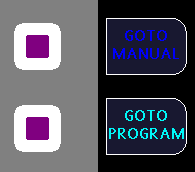
\includegraphics[width=.3\linewidth]{screen-captures/alarms-nav}
	\caption{Alarm Screen Navigation}
	\label{fig:alarm-nav}
\end{figure}
\begin{list}{$\diamond$}{}
	\item \textbf{GOTO MANUAL} Navigate to Manual Screen.
	\item \textbf{GOTO PROGRAM} Navigate to Cut Program Screen.
\end{list}

\paragraph*{\textbf{\LARGE \textcolor{blue}{i}}}
The Menu Key located on the terminal at the lower left below the FKey's, will return the Operator to the Main Screen, from all other screens.\\
\begin{minipage}{4cm}
	\begin{picture}(20,70)
	
\includegraphics[width=.5\linewidth]{screen-captures/menu}
	\end{picture}
\end{minipage}\begin{minipage}[]{11cm}
\paragraph{\textbf{\LARGE \textcolor{blue}{i}}} The Menu Key is pictured as it looks on the Terminal.
\end{minipage}
\pagebreak
\subsection{Alarm Message Display} Is the display area that details the Fault or Faults that have caused the Alarm. The Operator can use the detailed Fault information to take appropriate action to clear the Faulted condition. The \textbf{\textit{Alarm Message Display}} will scroll through the Fault Details that are currently active. Some Faults will be interrelated and the action of clearing one will often clear other related faults.
\begin{figure}
	\centering
	
\includegraphics[width=.5\linewidth]{screen-captures/alarm-msg-cntr}
	\caption{Main Screen Message Centre}
	\label{fig:alarm-msg-cntr}
\end{figure}
The \textit{Alarm Message Centre} shown in Figure 2.3 will display Alarm messages for the Operator. If more than one message is active the display will scroll through all messages continuously on a timed basis automatically. The Operator is not required to initiate any message change, but is required to acknowledge a message in order to clear the related Fault.
\\
\\
\\
\\
\\
\\
\\
\\
\\
\\
\\
\\
\\
\\
\\
\\
\\
\\
\\
\\
\\
\\
\\
\pagebreak
\subsection{Alarm Reset} The \textbf{\textit{Alarm Reset}} pushbutton is how the Operator acknowledges clearing a Fault. The Operator \textbf{must} acknowledge \textbf{all} Faults in order to clear them. All Faults must be cleared before the Operator can change the Saw into \textit{Auto Mode}. 
\begin{figure}
	\centering
	
\includegraphics[width=.3\linewidth]{screen-captures/alarms-reset}
	\caption{Alarm Reset Pushbutton}
	\label{fig:alarm-reset}
\end{figure}
\paragraph*{\textbf{\LARGE \textcolor{blue}{i}}}The details of the Fault which is causing the Alarm will be displayed in the \textbf{\textit{Alarm Message Display}}. The Operator can use this information as a guide to clearing the Faulted condition. Manual operation of the Saw is allowed under most Faulted conditions.
\paragraph*{\textbf{{\LARGE \textcolor{red}{!}}}}A fault that is triggered must be cleared and acknowledged in order to be able to run an automatic cut program on the saw. All faults are programmed to help the Operator prevent damage to the saw through normal use. The surrounding work area, and it's upkeep and cleaning can have an affect on Saw operations. It is the Operators responsibility to ensure the area is kept clutter free and the equipment travel paths are relatively clean.
\section{Faulted Conditions, Alarms, and the Operator} A machine as complex as a gantry rock cut saw, can have Faulted conditions arise from many areas of it's operation envelope.The severity of an alarm is a direct result of the severity of the Faulted condition that triggered the alarm. Therefore, it should come as no surprise to the Operator that some Faulted conditions are severe enough to prevent manual operation of part or all of the saw. The drives that move the Long, Cross, and Vertical axii of the saw are one such set of components that can have Faulted conditions that cripple the saw operation. Rectifying the condition that triggered the Fault is the one sure fired method of ensuring problem free operation of the saw. The Gantry Rock Cut Saw is a machine that works under harsh conditions. As such, it is to be expected that components will wear as the saw is used. This includes electrical and electronic components as well as the mechanical parts. After time, heavily loaded electrical components, such as saw motors, will suffer degradation of critical parts under stress. The Operator can note that there will be performance losses under such cases, and more frequent Faults of overload type, such as motor stalling. This will continue and usually worsen until failure of the weak components occurs. Understanding how the machine operates under well maintained normal conditions is a great benefit to the Operator when it isn't operating as expected. Faults, and their frequency of occurrance, can help the Operator note a trend towards component failure. This can lead to better maintenance cycles through preventative measures, reducing downtime and scrap as a direct consequence. Some Fault conditions may never be observed by the Operator directly, whether they are masked by another Fault condition or only occur under certain maintanence steps. An example of such a Fault condition is the Communication Network(s) used in the Control System Architecture. If the communication fails in a part that feeds information to the HMI (from the PLC), the error couldn't be displayed. This is a moot point under that specific Fault condition since there would be no screen navigation or control capabilities either, and the Operator would be aware a problem exists as a consequence. If communication is lost to the Drives Network for instance, the Faulted condition would be announced and the Operator would have \textit{Manual} mode capabilities. Trying to \textbf{\textit{Cycle Start}} an \textit{Auto} cycle without first entering in a correct cut program, is a Faulted condition that will trigger an alarm. The Operator would acknowledge such an Alarm by pressing the \textbf{\textit{Reset}} pushbutton on the \textbf{\textit{Alarms Screen}} to continue, then enter a valid cut program before trying to start another automatic cycle. Just like the Operator Message Centre on the Main screen, the Alarm Message Centre on the Alarms Screen is there for the Operator Information to assist in daily operations. Alarms can be expected to occur regularly during normal use. 
